\documentclass[a4paper,11pt]{article}

% set length of paper. put 'true' before unit like 31mm = 30truemm.
\usepackage[top=25truemm,bottom=25truemm,left=23truemm,right=23truemm]{geometry}
% set font to 'Times'
\usepackage{times}
% multi column
\usepackage{multicol}
\usepackage{color}
\usepackage[dvipdfmx]{graphics}
\usepackage{amsmath,amssymb}
\usepackage{bm} % italic bold (vector)
\usepackage{authblk} % author
\usepackage{fancyhdr} % header and footer
\usepackage{graphicx}
\usepackage{ascmac}
\usepackage{caption}
\usepackage{tikz}
\usepackage{here}
\usepackage{wrapfig} % 画像にテキストを回り込ませる
\usepackage{listings} % source code
\usepackage[version=3]{mhchem} %chemical equatio
\usepackage{titlesec} % relates to section

% settings of section and subsection
%\makeatletter
%\def\section{\@startsection {section}{1}{\z@}{0.1ex plus 2ex minus -.2ex}{0.1ex plus .2ex}{\normalsize\textbf}}
%\def\subsection{\@startsection {subsection}{1}{\z@}{0.1ex plus 2ex minus -.2ex}{0.1ex plus .2ex}{\normalsize\textbf}}
%\makeatother
%\pagestyle{empty}
%
%\setlength{\textwidth}{\fullwidth}
%\setlength{\texthight}{40\baselineskip}
%\addtolength{\texthight}{\topskip}
%\setlength{voffset}{-0.55in}
%
% キャプションの設定
\captionsetup[figure]{format=plain, labelformat=simple, labelsep=space, font=footnotesize}
\captionsetup[table]{format=plain, labelformat=simple, labelsep=space, font=footnotesize}
\renewcommand{\figurename}{Figure}
\renewcommand{\tablename}{Table}
%
% setting of source code
\lstset{
    basicstyle={\scriptsize\ttfamily},
    breakindent = 30pt,
    stringstyle={\scriptsize\ttfamily},
    basicstyle={\ttfamily},
  identifierstyle={\small},
  commentstyle={\smallitshape},
  keywordstyle={\small\bfseries},
  ndkeywordstyle={\small},
  stringstyle={\small\ttfamily},
  frame={tb},
  breaklines=true,
  columns=[l]{fullflexible},
  numbers=left,
  xrightmargin=0zw,
  xleftmargin=3zw,
  numberstyle={\scriptsize},
  stepnumber=1,
  numbersep=1zw,
  keepspaces=true,
  lineskip=-0.5ex,
}
% document
\begin{document}
% START DOCUMENT
%
% HEADER
\begin{center}
  % title, author
  {\fontsize{16pt}{16pt}\selectfont Numerical Analysis assignment No. 3\\}
  \vspace{16pt}
  \fontsize{10.5pt}{12pt}\selectfont
  B6TB1505 Daichi HAYASHI (Ohnishi Lab.)\\
  \vspace{10.5pt}
  Oct. 24th, 2019.\\
  \vspace{-2mm}
\end{center}

\section{Assignment Content}
To investigate $\Delta x$ dependence of the Trapezoid method and the Simpson$~\frac13$ method.

The governing equation (exact solution) is
\begin{equation}
	I = \int_{3.1}^{3.9} \dfrac1x \mathrm{d}x = \ln\left|\dfrac{3.9}{3.1}\right| = 0.229574441645...
\end{equation}

\section{Resultsit and Discussions}
The results of both methods is shown as Table 1. I used Python code which was distributed in the class. And I investigated at	 $\mathrm{imax}= 9,\ 51,\ 81,\ 201,\ 401,\ 801,\  8001,\ 80001$.

\begin{table}[H]
\centering
\caption{Results}
\begin{tabular}{lllcc}
  $\Delta x$& $\log(\Delta x)$ & imax & $\log (\varepsilon)$ of the Trapeziod & $\log (\varepsilon)$ of the Simpson 1/3 \\
  \hline\hline
  0.1 & -1.0 & 9 & -4.50 & -7.67 \\
  0.016 & -1.80 & 51 & -6.09 & -10.8 \\
  0.01 & -2.0 & 81 & -6.50 & -11.7 \\
  0.004 & -2.40 & 201 & -7.29 & -13.3 \\
  0.002 & -2.70 & 401 & -7.89 & -14.5 \\ \hline
  0.001 & -3.0  & 801 & -8.50 & -16.1 \\
  0.0001 & -4.0 & 8001 & -10.5 & -15.5 \\
  0.00001 & -5.0 & 80001 & -12.5 & -16.0
\end{tabular}
\end{table}
The last 3 lines from the result of the Simpson method (under the single line), there is no decreasing of error. This is highly possible to be Machine Zero. Therefore, I don't plot the last 3 lines of result. I use just the 5 lines above.

From the 5 results, I made fitting line by using Least–squares method. In the method, the fitting line is written by $y = Ax + b$, and the parameter $r$ is Correlation coefficient. The fitting result is shown as Table 2. Since both $|r| > 0.999$, the fitting is right.

\begin{table}[H]
\centering
\caption{Fitting line parameters}
\begin{tabular}{c|cc}
   & Trapezoid & Simpson 1/3 \\
  \hline
  A & 1.994 & 4.028 \\
  B& -2.505 & -3.618 \\
  r& 0.999995 & 0.99988 
\end{tabular}
\end{table}

And plot result and fitting line are shown in Figure 1. From these result, the Simpson 1/3 method's slope is 2 times steeper, so Simpson 1/3 converges faster than Trapezoid.

\begin{figure}[H]
	\centering
	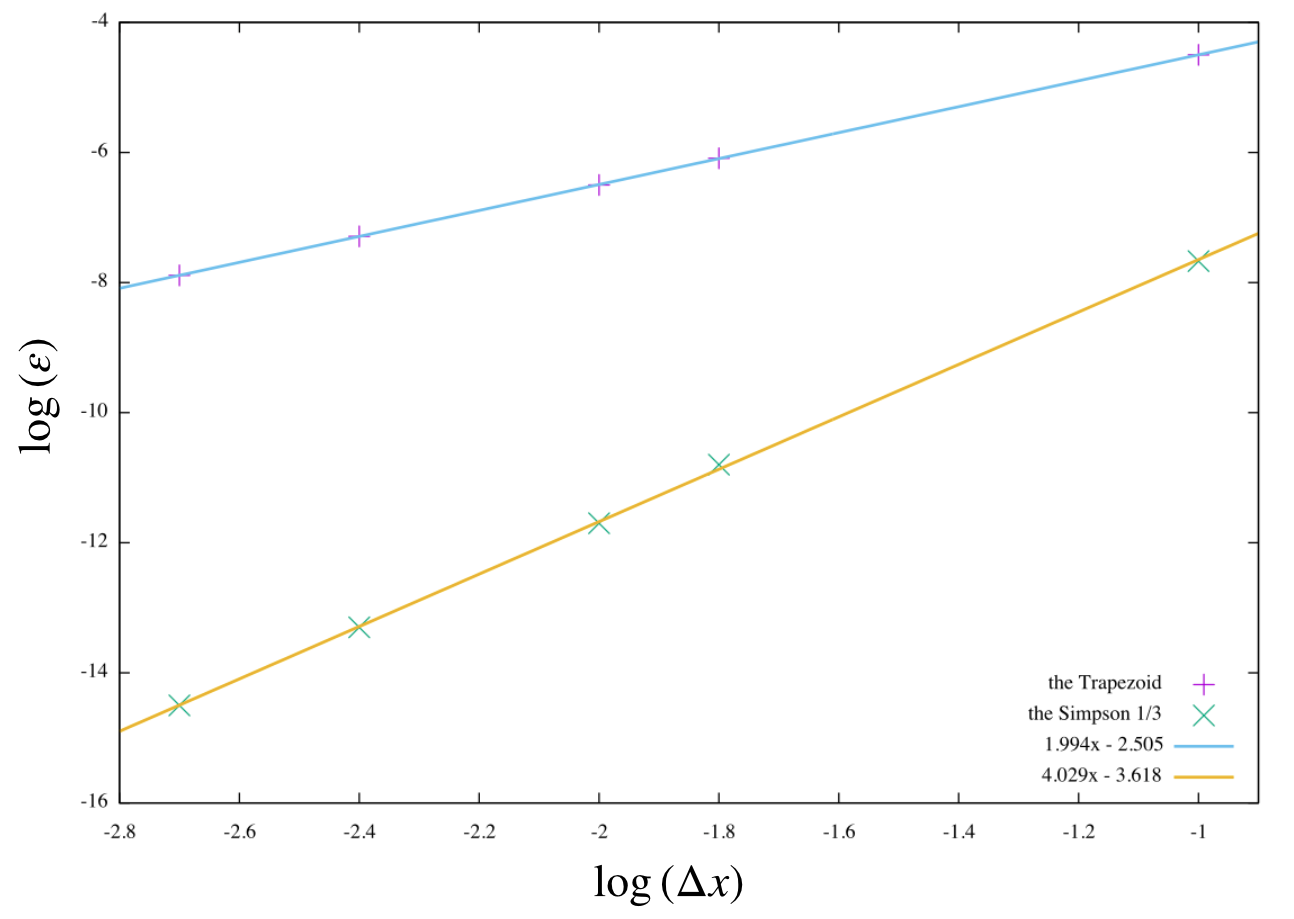
\includegraphics[width=12cm]{plot.png}
	\caption{Plots from results and fitting line.} 
\end{figure}


%
% END OF DOCUMENT
\end{document}
